\documentclass[runningheads]{llncs}

\usepackage[T1]{fontenc}

\usepackage{graphicx}

\begin{document}

\title{Modular IDE}

\author{Nils Michael Fitjar\inst{1,2}
}

\authorrunning{Nils Michael Fitjar}

\institute{Western Norway University of Applied Sciences\\
\email{798183@stud.hvl.no}
 \and
University of Bergen\\
\email{nfi005@uib.no}
}

\maketitle
\begin{abstract}
This paper introduces a modular Integrated Development Environment (IDE) for experimental programming languages,
addressing limitations in traditional IDEs. While standard IDEs are crucial in software development,
their support for experimental languages is often inadequate. This project proposes a modular IDE to extend its
lifespan and enhance support for experimental languages. Analyzing the essential features of traditional IDEs and
the need for adaptability to new paradigms and tools. Magnolia, a generic programming language developed at UIB,
serves as a case study, highlighting its unique characteristics and the necessity for a specialized IDE.
The primary research question explores how modularization facilitates the design and implementation of experimental
programming languages. Specific modules or plugins tailored for experimental languages, including
Abstract Semantic Representation (ASR) Transformation, Term Algebras, MoA translation,
and Syntactic Theory Functor (STF), are outlined. These plugins will be implemented to validate the
modularized IDE's functionality, with a focus on the ASR Transformation module.

\keywords{Modularization \and IDE \and Magnolia.}
\end{abstract} 

\chapter{Introduction}

Standard \gls{ide}s are indispensable tools in modern software development,
offering features like early bug reporting, project outline visualization, code
highlighting, and code completion, however, these \gls{ide}s may not adequately
support the unique demands of experimental programming languages. Experimental
languages could introduce new concepts like \gls{asr} Transformation, Term
Algebras, \gls{moa}, \gls{stf}, or other novel programming features. These are
concepts from the academic community, and are not common in \textit{mainstream}
languages, and as such, have little to no support in modern \gls{ide}s. To solve
this, researchers need ad hoc solutions for existing \gls{ide}s, adding the
needed functionality to test out their language features. If this ad hoc
solution is too extreme; outside the standard functionality supported by the
developers of the \gls{ide}, it might be short-lived. As the \gls{ide} is
maintained, updated and improved, the features used to solve the niche needs of
the experimental language might be deprecated.

However, if the \gls{ide} has integrated support for extending the standard
functionality of the application, then the ad hoc solution will be more stable.
Such a system is known by many names. Plug-in architecture, exstension
\gls{api}, or add-on system, to name a few. The common factor amongst these
systems, is that some component, be it a plug-in, an exstension, an add-on, or a
module, can extend the functionality of the application. This is a modular
approach to extending the lifetime of an application; extending its software
longevity. In many of these systems, said components, are composable,
allowing for multiple components to work together in a modular fashion to add
extra features to an application. This way of adding functionality to an
application is commonly used in \gls{ide}s.


\section{Modular Architecture}

A modular \gls{ide} would assist in these ad hoc solutions. Even if a new
feature from an experimental language is introduced, it is unlikely that this
feature has no relation to existing features, and as such, it is easier to
extend the application in such a manner to facilitate this new feature, with help of
existing modules. However, if it is the case that this feature is
paradigm-shifting, then there will still be existing functionality that can be
used, re-used or extended to facilitate this.

\begin{hyp} \label{hyp:modular}
  When an application is designed to be modular from the start, then features
  not thought of, by the original developers can be integrated into the
  application, and be stable. If an experimental research language introduces
  some paradigm shifting concept, then this can easily be tested in a modular
  \gls{ide}.
\end{hyp}

\section{Zero-core Application}

Taking the modular architecture design to the extreme, the core application has
no base features, everything is enabled by an external module. We call such a
highly modular application, a \textit{zero-core} application. To qualify for a
\textit{zero-core} application, the default application has no functionality;
everything is acquired by modules. Such a design facilitates a modular approach,
enabling a module-developer to only focus on the functionality they want to
extend, not the entire core.

\section{Thesis Outline}

Traditional \gls{ide}s encompass essential features such as syntax highlighting,
code navigation, and hover-help, all of which play a crucial role in the
software development process. However, their limitations become apparent when
working with experimental languages. This paper advocates for modularization and
composability as key design principles, demonstrating their ability to extend
the operational lifespan of software by allowing for ease-of adoption to new
paradigms and tools. The discussion revolves around Magnolia, an experimental
research programming language developed by \gls{bldl} at the University of
Bergen. Magnolia is a way to experiment with novel language features. It will
therefore be a case study illustrating the need for a specialized \gls{ide}. To
achieve this in a sufficient manner, a more specialized \gls{ide} is required.

The focus point of this paper is to design a zero-core architecture, to develop
and implement a modular \gls{ide}, where the target language will be Magnolia.

In chapter \ref{cha:background}, we will introduce Magonlia, and features this
language introduces that are difficult to encompass using standard \gls{ide}s.
In chapter \ref{cha:ide} we will explore the use case of the afformentioned
\gls{ide}, focusing on the different users of such an application. Chapter
\ref{cha:impl} the design and implementation of the \gls{ide}, mentioning
different designs that were considered, and some challanages that were
encountered.


\chapter{Background} \label{cha:background}

\section{Magnolia}

Magnolia is an experimental research language being developed \gls{bldl} at the
University of Bergen. Magnolia is designed to support a high level of
abstraction and ease of reasoning. This is achieved by \textit{concepts},
\textit{axioms}, \textit{satisfaction}, and \textit{implementations}.

\subsection{Magnolia Concept}

Something, Something, \dots, concepts declare types, functions and properties
which those functions need to uphold. A simple example of this would be a
concept for addition with natural numbers.

\begin{center}
  \lstinputlisting
    [ language=Magnolia
    , caption={Natural numbers (Magnolia)}
    , label=lst:nat
    ]{./code/magnolia-nat.mg}
\end{center}

In the listing \ref{lst:nat}, we are specifying concept called
\textit{NaturalNumbers}, which declares a type \textbf{N}, and three methods
that act upon the type \textbf{N}. We have the function, (also called a
constructor), \textbf{zero}, which takes zero arguments, and should return
something of type \textbf{N}. With this constructor, we can instantiate our
numbers. To get new numbers, we have the function \textbf{succ}, which should
give the \textit{succ}essor to the passed number. That way, we can represent $0$
as \textbf{zero()}, $1$ as \textbf{succ(zero())}, and $2$ as
\textbf{succ(succ(zero()))}. The final function, is an infix operator. $+$ takes
two arguments, of type \textbf{N}, and returns an \textbf{N}. Of course, this
should be interpreted as addution, meaning \textbf{succ(zero())} $+$
\textbf{succ(succ(zero()))} $=$ \textbf{succ(succ(succ(zero())))}, or using
numbers: $1 + 2 = 3$. Finally, the last statement in the concept, is an axiom,
stating that given any $a$, if we add \textbf{zero()} to $a$, we should get $a$.
However, this interpretation depends on our implementation
of the concept.
\todo{Add more examples showcasing what is needed from a Magnolia IDE}
\todo{Renaming}
\todo{Showing all imports are DAG's}

\subsection{Magnolia Implementation}

As one can see in listing \ref{lst:impl}, we have implemented the concept
specified in \ref{lst:nat}, by using concrete values for \textbf{N}. There is an
implementation for all the functions, giving us the functionality we set out to
specify with our concept, but there is nothing stopping us from straying away
from the specification, by implementing it incorrectly. As can be seen in
listing \ref{lst:impl-wrong}.
\todo{Add more examples showcasing what is needed from a Magnolia IDE}

\begin{center}
  \lstinputlisting
    [ language=Magnolia
    , caption={Natural numbers implementation (Magnolia)}
    , label=lst:impl
    ]{./code/magnolia-add.mg}
\end{center}

\begin{center}
  \lstinputlisting
    [ language=Magnolia
    , caption={Invalid implementation (Magnolia)}
    , label=lst:impl-wrong
    ]{./code/magnolia-add-wrong.mg}
\end{center}

Here we have implemented our addiction operator in such a way, where it breaks
our axiom. This is where the \textit{satisfaction} comes in, it is what ties the
concept and implementation together, by ensuring our axiom are upheld.


\subsection{Magnolia Satisfaction}

\begin{center}
  \lstinputlisting
    [ language=Magnolia
    , caption={Satisfaction of the natural numbers (Magnolia)}
    , label=lst:sat
    ]{./code/magnolia-add.mg}
\end{center}

Something, Something, \dots, implementations of concepts need to uphold the
axioms declared in the concept being implemented. This is done by using an
external SMT-solver. Satisfaction, babay
\todo{Cite Beate maybe?}

\todo{
  Expand, maybe exploring generic concepts, axioms and implementation, noting
  how a developer would use Magnolia?
}

\subsection{Mathematics and Programming}

Mathematics is everywhere, and useful. It's not always easy to notice this, but
one thing that helps, is knowing the names of the concepts one encounter. One
can easily understand that knowing simple operations like addition,
multiplication, etc. is useful but for more abstract mathematics, this is
harder. An example of this is abstract algebra, which is the study of algebraic
structures, which are structures that are very common in programming. A
programmer will use these structures more often than not, knowingly or
unknowingly, and a good programmer will explicitly seek these structures out.

An important aspect of development, is logging. Knowing what actions have taken
place is an essential tool when hunting down bugs. A common way to structure
logs, would be composing logs, depending on when they occurred. As a concrete
example, let's say we are making a text editor, and are in the need of a logging
manager, which, among other things, should compose different log statements.
Assuming we have some type \textbf{Log(A)}, where there the type \textbf{A}, is the
result of the computation a given function, we want to be able to compose
different, related, computations. But, importantly, the order of composition
of the \textbf{Log(A)}-type matters. Representing the composition of the
\textbf{Log(A)}-type as $\odot$, doing, and letting $a, b, c$ be of type
\textbf{Log A}:

\begin{equation}
  a \odot \left ( b \odot c \right ) = \left ( a \odot b \right ) \odot c
\end{equation}

Now we have a good logger, as the logs of the entire call stack is available for
us to read when something goes wrong. Moving on, a good feature of a text
editor, is being able to undo and redo actions. These are the actions that a
user can do:

\begin{itemize}
  \item Insert text at a position
  \item Delete text from a position
  \item Redo an action
  \item Undo an action
\end{itemize}

Same as in the logging example, composing is a reasonable thing to implement,
and should result in another action. Similarly, the order matters; deleting text
and then inserting, is not the same as inserting and then deleting. But what is
different, is that we also want the \textit{inverse} of an action, so for every
action we want an opposite action that undos an action. Then our composition of
actions looks different. Say, $a$ is some action, and $c$ is some opposite
action, then our composition looks like this:

\begin{equation}
  a \odot c = U
\end{equation}

Where $U$ is an action representing \textit{no-operation}. This could be
inserting the empty string at any position, deleting the empty string at any
position, or redoing or undoing any of the aforementioned actions.

Both of these examples are relatively easy to implement, but harder to verify,
or satisfy our properties; that the \textit{logic} holds. The following are
examples of the logging and editor examples in Java, Rust, and Magnolia
respectively.
\todo{rewrite}

\subsection{Logging example in Java, Rust, and Magnolia}

\todo{Expand}

\begin{center}
  \lstinputlisting
    [ language=Java
    , caption={Logging structure (Java)}
    , label=lst:jlogging]{./code/logging.java}
\end{center}

\begin{center}
  \lstinputlisting
    [ language=Rust
    , caption={Logging structure (Rust)}
    , label=lst:rlogging]{./code/logging.rs}
\end{center}

\begin{center}
  \lstinputlisting
    [ language=Magnolia
    , caption={Logging structure (Magnolia)}
    , label=lst:mlogging]{./code/logging.mg}
\end{center}

\subsection{Editor example in Java, Rust, and Magnolia}

\todo{Expand}

\begin{center}
  \lstinputlisting
    [ language=Java
    , caption={Editor structure (Java)}
    , label=lst:jeditor]{./code/editor.java}
\end{center}

\begin{center}
  \lstinputlisting
    [ language=Rust
    , caption={Editor structure (Rust)}
    , label=lst:reditor]{./code/editor.rs}
\end{center}

In Magnolia, however, this can be enforced on the \textit{interface}-level.
\todo{Rewrite}

\begin{center}
  \lstinputlisting
    [ language=Magnolia
    , caption={Editor structure (Magnolia)}
    , label=lst:meditor]{./code/editor.mg}
\end{center}

The interesting thing about these two structures, is that they are similar,
even though they are used for two different things. Both the logging example,
and the text editor example, are some binary operation over some set. In the
first example, our set was all different log statements of the type
\textbf{Log A}, and composing these logs, gave us another \textbf{Log A} type.
While in the second example, we were working on the set of actions, which we
could compose, which also gave us another action, but we also had an action
representing no-operation, and an \textit{inverse} operation, undoing an action.
This is related to mathematics, specifically abstract algebra, the study of
algebraic structures.

\subsection{Abstract Algebra}

In the first example, we are working with a \textit{semigroup}, and in the
second example, we are working with a \textit{group}. These are known as
algebraic structures, which is just some set, with a binary operation, and some
property on that binary operation. The trivial example, is known as
\textit{magma}, and is defined by \ref{def:magma}. The closure \ref{def:closed}
simply specifies that we only work with one set.

\begin{definition}[Closure] \label{def:closed}
  For a set $M$, with a binary operation $\oplus$,
  $\forall a, \forall b, \exists c \in M$, such that
  $a \oplus b = c$.
\end{definition}

\paragraph{Closure} Addition with the integers, ($\mathbb{Z}$), is a kind of
  closure, as per the definition \ref{def:closed}, since no matter what integer
  you put into the equation, you will still get a positive integer. And since
  this is the only requirement a magma has, this example is also a magma.

\begin{definition}[Magma] \label{def:magma}
  A magma is a set $M$, with a binary operation $\oplus$, which is
  \textit{closed} by definition \ref{def:closed}
\end{definition}

We can \textit{extend} the definition of magma, by adding associativity on the
binary operation. The definition \ref{def:assoc}, as shown in the examples,
simply specifies that the order we evaluate our composition matters.

\begin{definition}[Associativity Law] \label{def:assoc}
  For any binary operation $\oplus$, on a set $M$, $a, b, c \in M$.
  $a \oplus \left ( b \oplus c \right ) = \left ( a \oplus b \right ) \oplus c$,
  must hold.
\end{definition}

This associativity gives us a semigroup, as shown in the definition
\ref{def:semi}, which is the structure that we modeled in our logging example.

\begin{definition}[Semigroup] \label{def:semi}
  A semigroup is a set $M$, with a binary operation $\oplus$, and $\oplus$ must
  uphold the definitions \ref{def:closed} and \ref{def:assoc}.
\end{definition}

\paragraph{Semigroup} Multiplication with the positive integers, ($\mathbb{N}$), is
  associative, since no matter where we put parentheses; what order we
  evaluate this equation: $2 * 3 * 4$, we will get the same answer.

By simply requiring the identity law (\ref{def:ident}), we get a
monoid (\ref{def:monoid}), and adding the inverse law
(\ref{def:inv}), we get a group.

\begin{definition}[Identity Law] \label{def:ident}
  For any binary operation $\oplus$, on a set $M$,
  $\forall a, \exists U \in M$, such that
  $a \oplus U = a$, and $U$ is unique.
\end{definition}

\begin{definition}[Monoid] \label{def:monoid}
  A monoid is a set $M$, with a binary operation $\oplus$, and $\oplus$ must
  uphold the definitions \ref{def:closed}, \ref{def:assoc}, and \ref{def:ident}.
\end{definition}

\paragraph{Monoid} To make a monoid, we can choose the binary operation to be
  $\times$, and our set to be the natural numbers, ($\mathbb{N}$). We know addition
  is closed, and associative, so choosing $U = 1$, we get a monoid. Any number
  from our set $\mathbb{N}$ multiplied with $1$, gives us the number we choose.

\begin{definition}[Inverse Law] \label{def:inv}
  For any binary operation $\oplus$, on a set $M$,
  $\forall a, \exists U \in M$, such that
  $a \oplus U = a$, and $U$ is unique.
  And $\forall a, \exists b \in M$, such that $a \oplus b = U$, and the mapping
  for $a \to b$ is one-to-one.
\end{definition}

\begin{definition}[Group] \label{def:group}
  A group is a set $M$, with a binary operation $\oplus$, and $\oplus$ must
  uphold the definitions \ref{def:closed}, \ref{def:assoc}, \ref{def:ident},
  and \ref{def:inv}.
\end{definition}

The definition \ref{def:group}, of course is identical to the structure we used
to model undo-redo, in our text editor example. To avoid common mistakes when
implementing these structures, it would behoove a developer if they could encode
these properties in something like an interface or a trait, however, this is not
possible in either Java nor Rust.
\todo{Rewrite this}

\todo{Rewrite this to better fit the previous section}

\subsection{Java: Magma to Group}

This structure not could be implemented in something like Java, an
Object-Oriented Language, as shown in listings \ref{lst:jmagma},
\ref{lst:jsemigroup}, \ref{lst:jmonoid}, and \ref{lst:jgroup}. Note the empty
interfaces; there is nothing that enforces the different laws on the properties.
This can only be done by unit testing, which is not enforced on a consumer of
the \gls{api}.

\begin{center}
  \lstinputlisting
    [ language=Java
    , caption={Magma concept (Java)}
    , label=lst:jmagma]{./code/magma.java}
\end{center}

\begin{center}
  \lstinputlisting
    [ language=Java
    , caption={Semigroup concept (Java)}
    , label=lst:jsemigroup]{./code/semigroup.java}
\end{center}

\begin{center}
  \lstinputlisting
    [ language=Java
    , caption={Monoid concept (Java)}
    , label=lst:jmonoid]{./code/monoid.java}
\end{center}

\begin{center}
  \lstinputlisting
    [ language=Java
    , caption={Group concept (Java)}
    , label=lst:jgroup]{./code/group.java}
\end{center}

\subsection{Rust: Magma to Group}

\todo{Expand}

\begin{center}
  \lstinputlisting
    [ language=Rust
    , caption={Magma (Rust)}
    , label=lst:rmagma]{./code/magma.rs}
\end{center}

\begin{center}
  \lstinputlisting
    [ language=Rust
    , caption={Semigroup (Rust)}
    , label=lst:rsemigroup]{./code/semigroup.rs}
\end{center}

\begin{center}
  \lstinputlisting
    [ language=Rust
    , caption={Monoid (Rust)}
    , label=lst:rmonoid]{./code/monoid.rs}
\end{center}

\begin{center}
  \lstinputlisting
    [ language=Rust
    , caption={Group (Rust)}
    , label=lst:rgroup]{./code/group.rs}
\end{center}

\subsection{Magnolia: Magma to Group}

In Magnolia, however, this can be enforced on the \textit{interface}-level. The
example code shown in listing \ref{lst:magma}, showcases a concept
representation a binary operation, which has one function, \textit{binop}, which
takes in two values of type \textit{T}, and returns \textit{T}. Note that the
actual implementation of this function is missing. This is because a concept
encodes the properties of a users code. The actual implementation of the
binary function needs to uphold the properties of the concept that is
being implemented. Note that this is unlike the Java and Haskell example, in
which we have no way to encode the property of our binary function. So any
consumer of our \gls{api} would not be explicitly bound to our restriction of
the associativity law \ref{def:assoc}, identify law \ref{def:ident}, and the
inverse law \ref{def:inv}, required by semigroup and group. The closure
definition, \ref{def:closed}, however, can be encoded by the type system in Java
and Haskell.

\begin{center}
  \lstinputlisting
    [ language=Magnolia
    , caption={Magma (Magnolia)}
    , label=lst:magma]{./code/magma.mg}
\end{center}

In the example code shown in listing \ref{lst:semigroup}, the \textit{magma}
concept has been expanded upon, still following the same rules as before, but
with the added property of associativity.

\begin{center}
  \lstinputlisting
    [ language=Magnolia
    , caption={Semigroup (Magnolia)}
    , label=lst:semigroup]{./code/semigroup.mg}
\end{center}

\begin{center}
  \lstinputlisting
    [ language=Magnolia
    , caption={Monoid (Magnolia)}
    , label=lst:monoid]{./code/monoid.mg}
\end{center}

\begin{center}
  \lstinputlisting
    [ language=Magnolia
    , caption={Group (Magnolia)}
    , label=lst:group]{./code/group.mg}
\end{center}

So Magnolia facilitates reuse, and extension of logic. \todo{expand}

\section{Reusable Software}

One of the most important features in any programming language, is the notion
of \textit{reusability}. From the invention of the GO-TO-statement,
to functions, and external libraries, being able to reuse existing software is
an important tool for a developer. It avoids \textit{re-inventing the wheel}, as
common functionality can be externalized and reused in several different places.
\todo{Can probably expand this by going more in depth}

\subsection{Reuse in Magnolia}

Reusability is also an important feature in Magnolia, but this reusability is in
the entire language. In libraries in other languages, functions are reused, in
an attempt to avoid common logical mistakes, but these mistakes could still be
there, hiding in plain view. In Magnolia, one can re-use the \textit{logic} of a
\todo{Expand}
function. The logging and group example can be rewritten using Magnolia concepts
as shown in listing \ref{lst:logging} and \ref{lst:editor} respectively, by
reusing the concepts we created for semigroup in listing \ref{lst:semigroup} and group
in listing \ref{lst:group}.

\begin{center}
  \lstinputlisting
    [ language=Magnolia
    , caption={Logging example (Magnolia)}
    , label=lst:logging]{./code/logging.mg}
\end{center}

\begin{center}
  \lstinputlisting
    [ language=Magnolia
    , caption={Editor example (Magnolia)}
    , label=lst:editor]{./code/editor.mg}
\end{center}

Here we have used the \textit{renaming} of concepts in Magnolia, where we can
rename types and functions to be more specific, for the specialized use case the
concept is reused in.

\subsection{Software Longevity}

Most examples of \textit{popular} software, are open source, like \gls{vim}.
\gls{vim} is a text editor which has been in use since 1991. There are several
factors behind this success, but the ones being highlighted here, are due to its
extensibility and due to it being open-sourced. Being open sourced, allows for a
rotating cast of maintainers, ensuring the core application has the features its
users wants. The users of \gls{vim} can be split into two categories,
\textit{standard users}, and \textit{module developers}. \gls{vim} has an
extensive module ecosystem, which can extend \gls{vim}s functionality from a
text editor, to a fully fledged \gls{ide}.
\todo{Currently, a weak argument for modularity}
\todo{Mention Eclipse and IntelliJ here as well?}

\section{Integrated Development Environment} \label{sec:ide}
\todo{Turn each paragraph into a subsection?}

An \gls{ide}, aids a developer, as all the needed tools for development are
\todo{Mention the tools, and how devs had it before.}
integrated into one application. There are two different kinds of \gls{ide}s,
generic and specialized. \todo{Source}

A specialized \gls{ide} is one targeted towards a specific language, like
Eclipse, (reference?), or IntelliJ (reference?), which target Java/JVM. It
contains specialized features like the following:
\todo{
  Rewrite this because Eclipse, while generic, has plugin support which, allows
  it to support different languages, as does IntelliJ.
}

\paragraph{Syntax Highlighting} Highlighting important keywords, identifiers
and more, makes the language easier to read for the developer, allowing them to
spot easy to miss errors, like misspelling of keywords, functions, and
variables.

\paragraph{Code Autocompletion} Suggesting keywords, method names or even entire
code snippets, is a powerful tool an \gls{ide} can have. This is possible to
achieve, in some form, without being specialized, by for example, suggesting
text that already exist in the document, but is most useful if it is
specialized, and can suggest built-in methods. This allows a developer to not
having to remember exactly how methods are named, is the method to split a
string by some delimiter, \textit{split\_by} or \textit{split\_on}? As long as
the developer writes \textit{split}, the correct method name will be suggested.

\paragraph{Go-To-Definitions} Being able to quickly navigate to methods and read
their implementation is a useful tool for a developer, as less time has to be
spent navigating the project structure, to figure out where some method was
implemented, and more time can be spent actually developing.

\paragraph{Pretty Printing/Formatting} Following the languages style guide.
\todo{Expand, add examples like with Rust}

\paragraph{Boilerplate Code Generation} For unit tests, getters and setters,
(where relevant), and similar.

A lot of these features are possible due to \gls{lsp} which allow for a
standardized way for compilers to give code-support to \gls{ide}'s.

A generic \gls{ide} contains the features that are common among development in
any programming language, like:

\paragraph{File Explorer} Most project nowadays is larger than one file, so
being able to visualize the project in a tree-like-structure, and navigate that,
is useful. This feature usually comes with the ability to manipulate the project
structure, by adding files, folders, moving files around, and deleting them.

But creating any \gls{ide} would still limit the lifetime of the \gls{ide}.
The best example of a long living active \gls{ide}, or, at least editor, is Vim
(source?). Vim is not a feature full editor, but it is simple, lightweight, and
works on any operating system. But most people use it, for how easy it is to
extend; Its lifetime has been greatly extended by the ease of modularization.
Any popular module for Vim is open-source, and therefore, if any module had an
active community around it, if the \textit{lead} developer of the module stopped
developing it, that community can continue to develop the module, either by
getting maintenance access to the repository, or by forking it. Ensuring the
lifetime of the module is extended.

\section{Module Architecture}

\todo{Talk about modules in IDEs}

A modular application, is an application which can be extended by other pieces
of software. This extensibility is useful as features that the original
developers of the application did not think about, can be added. If this module
architecture is well-designed, then this extension can be added without changing
the core application.

There are different ways an application can be extended. The most common one
uses so-called \textit{live-reload}, in which, if a module drastic changes the
functionality of an application, the application has to be restarted, or if it
is a \textit{minor} change, the module is simply loaded. This method is
extending the application during runtime, which is the method most users
expect. Another method would be \textit{compile-time-extension}, in which
modules are added before the application itself is compiled. There are some
advantages and disadvantage in all approaches.

Something, something \dots, in Eclipse modules extending modules is quite
common, using Eclipse Rich Client Platform. \cite{eclipseRcp}

\subsection{Compile Time Module}

\todo{Expand}
As an example, a standard user of any application will expect the application to
come bundled with all the needed functionality. This is best achieved with the
\textit{compile-time-extension} method, since the application can be installed
with the expected modules. A compile time module is usually made using the same
language as the core application.
\todo{Maybe mention it could be faster due to compiler optimalization?}

\subsection{Runtime Module}

\todo{Expand}

Runtime modules are usually also interpreted, but they can still be a
library, same as in a compile time module.

\subsection{Module Ecosystem}

\todo{Expand}
More modules == better, right?

In modern \gls{ide}s, with an extensive module architecture, there exists a
vast module ecosystem. From simple modules that change the color scheme, or
add file icons to more complex modules that add support for other languages.
A good variety of a module ecosystem can help ensure the longevity of an
\gls{ide}. In the table \ref{tbl:mod}, we can see that \gls{ide}s have an
extensive module architecture. \footnotemark

\footnotetext{
  \unskip Data found by looking at the marketplace\footnotemark for the modules,
  \unskip in order:
  \unskip \url{https://marketplace.eclipse.org/content/welcome-eclipse-marketplace}% Eclipse
  \unskip, \url{https://plugins.jetbrains.com/} % Intellij
  \unskip, \url{https://github.com/search?q=vim+plugin\&type=repositories} % Vim
  \unskip, \url{https://github.com/search?q=nvim+plugin\&type=repositories} % Nvim
  \unskip, \url{https://marketplace.visualstudio.com/search?target=VSCode\&category=All\%20categories\&sortBy=Installs} % vscode
}

\begin{table}[]
  \centering
  \caption{Module Ecosystem per \gls{ide}}
  \label{tbl:mod}
  \begin{tabular}{|l|l|}
    \hline
    \gls{ide} & Module count \\ \hline
    Eclipse & $\sim1200$ \\ \hline
    Intellij & $\sim9500$ \\ \hline
    \gls{vim} & $\sim11500$ \\ \hline
    Nvim & $\sim16100$ \\ \hline
    VS Code & $\sim71700$ \\ \hline
  \end{tabular}
\end{table}

\footnotetext{
  Nvim and Vim's marketplace is GitHub, so the results are found by searching
  GitHub for Nvim plugins and Vim plugins respectively, furthermore, all Vim
  plugins can be used by Nvim.
}

\subsubsection{Module Marketplace}

It is important to be able to get modules.

\todo{Mention the need for a module marketplace}

\subsection{Granularity}

When designing modules, the \textit{granularity} of the combined modules has to
be considered. As an example, if one where to extend the zero-core application
with the needed functionality for it to be considered an \gls{ide}, this could be
achieved by creating a singular module which does all the work. However, this
is not a modular approach, as if one wants to change some specific feature in
the \gls{ide}-module, one would have to re-create the whole module with that
specific feature implemented. Instead, if this functionality was granular,
that is to say, split into several modules, that together enable the needed
features, then it would be \textit{simpler} to modify the needed modules to
achieve the wanted feature.


\subsection{Module Family}

\todo{
  Redo this to be less specific, then add a specific section, which reflects
  what has been done
}

\begin{figure}
  \centering
  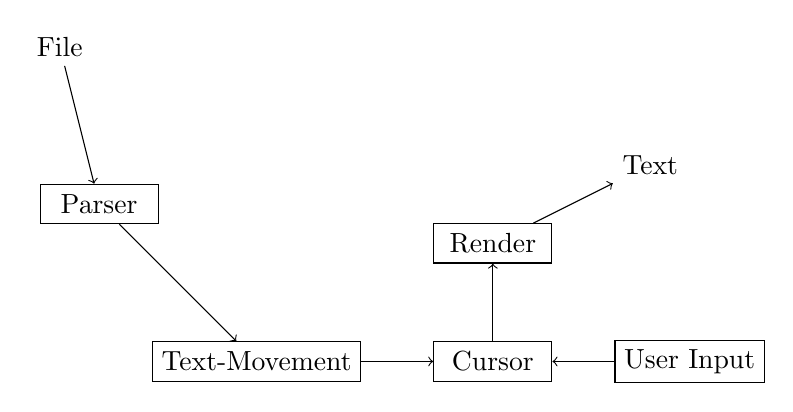
\begin{tikzpicture}
  % Nodes
  \node (file) [] at (-6, 3) {File};
  \node (parser) [rectangle, draw, minimum height=0.5cm, minimum width=1.5cm] at (-5.5, 1) {Parser};
  \node (text-movement) [rectangle, draw, minimum height=0.5cm, minimum width=1.5cm] at (-3.5, -1) {Text-Movement};
  \node (cursor) [rectangle, draw, minimum height=0.5cm, minimum width=1.5cm] at (-0.5, -1) {Cursor};
  \node (user-input) [rectangle, draw, minimum height=0.5cm, minimum width=1.5cm] at (2, -1) {User Input};
  \node (render) [rectangle, draw, minimum height=0.5cm, minimum width=1.5cm] at (-0.5, 0.5) {Render};
  \node (text) at (1.5, 1.5) {Text};
  % Arrow
  \draw[->] (file) -- (parser) node[midway, above] {};
  \draw[->] (parser) -- (text-movement) node[midway, above] {};
  \draw[<-] (cursor) -- (text-movement) node[midway, above] {};
  \draw[<-] (cursor) -- (user-input) node[midway, above] {};
  \draw[->] (cursor) -- (render) node[midway, above] {};
  \draw[->] (render) -- (text) node[midway, above] {};
\end{tikzpicture}

  \caption{Text Editor Module Family}
  \label{fig:textEditorSimple}
\end{figure}

In figure \ref{fig:textEditorSimple}, an input file is parsed to some structure
which is used to translate user actions, into cursor movements. The cursor being
the place in the file where text is written to by the user.

This is a feature that naturally shows up in a \textit{true} modular system. If
several modules together enable some feature, then those modules can be treated
as a singular module by an external module developer, depending on what they
want to extend.


\section{Language Workbench}

Language workbenches are environments for simplifying the creation and use of
computer languages. \cite{lwb}

\todo{Expand}

\section{Language Server}
\todo{Go more in depth about language server stuff}
The most important features in a modern \gls{ide} are possible due to the
\gls{lsp}. \gls{lsp} is a protocol for a language server and editor,
(the client), with which they communicate, allowing for many of the features
mentioned in section \ref{sec:ide}, and explicitly mentioned in table
\ref{tbl:ide}. \gls{lsp} being the standard since the 2020s, is a sign of
modularity being preferred, as now a single \gls{lsp} can be created, and used
across several different applications, like IntelliJ, VS Code and \gls{vim}.
While useful for \textit{standard} language, this is the limiting factor when it
comes to supporting experimental languages, as not only does a new set of
protocols need to be appended to a language server, the editor itself needs to
be changed to actually use these protocols. This creates a lot of work, for both
the \gls{ide} developer and for the compiler developer. Here is where a modular
approach can help both. If some new functionality or feature is added to the
experimental language, this off course means the compiler/interpreter has to be
expanded and/or modified, but for the \gls{ide}, a module could be added and/or
modified to utilize this change, instead of having to change the entire
application.

\begin{table}[]
  \centering
  \caption{\gls{ide} features enabled by \gls{lsp}}
  \label{tbl:ide}
  \begin{tabular}{|l|l|}
    \hline
    IDE Feature & \gls{lsp}-method \\ \hline
    Go to Declaration & textDocument/definition \\ \hline
    Go to Implementation & textDocument/implementation \\ \hline
    Auto-completion & textDocument/completion \\ \hline
    Hover & textDocument/hover \\ \hline
    Warnings & textDocument/publishDiagnostics \\ \hline
    Rename & textDocument/rename \\ \hline
  \end{tabular}
\end{table}

\section{Existing Magnolia IDE}

The current \gls{ide} for Magnolia \cite{baggeIde}, is a many-years-old version
of Eclipse, using modules and functionality from the core Eclipse application,
that has since been outdated. The \gls{ide}s lifetime was limited by a
dependency on external modules and features that where not maintained by the
\gls{ide}-developers. This meant that for future development of Magnolia, an
outdated \gls{ide} was needed, with outdated tooling. Furthermore, the Magnolia
\todo{This could be its own section, maybe?}
compiler was implemented as an Eclipse module, which means that development is
limited to Eclipse, and only Eclipse, as a developer cannot compile Magnolia
code without it.

Modularization will help to mitigate some of the issues with the current
Magnolia \gls{ide}. Instead of maintaining an entire application, the needed and
wanted features of the application can be maintained instead.

Experimental languages might have features which are not possible to be fully
used in current \gls{ide}s. This is also the case for the current Magnolia
\gls{ide}. The compiler for Magnolia, syntax highlighting, error reporting, and
hover-functionality are functionality made in the Eclipse \gls{ide}, by using
its plug-in architecture. Some of the functionality and plug-ins this
implementation used, have been deprecated in later version of Eclipse. This
means the Magnolia \gls{ide} is locked to an old version of Eclipse, which, as
time passes, increases the complexity of installation, as the surrounding
tooling and libraries needed by this version of Eclipse also becomes deprecated.
Currently, in INF220, at the university, two weeks are set aside for students to
be able to install it.

\section{Challenges imposed by Magnolia}

In most programming languages, any type has a singular definition, so invoking
the \textit{go-to-definition} endpoint implemented by an \gls{lsp} results in a
singular response. The actual response of the \gls{lsp} is a list, but this is
\textit{always} a singleton. However, in Magnolia a singular type could have
multiple definitions, and resolving this can be complex.

\subsection{Renaming}

As shown earlier, in Magnolia, one can make some concept, and reuse this concept
in another one. An example of this can be shown in listings \ref{lst:foo}, and
\ref{lst:bar}, where we have the concept \textit{Foo} being used in \ref{lst:bar}.
\todo{Make this true}
\todo{Add a non-empty-list example}

\subsection{Dependency Cycles}

Programming languages have different ways to avoid this problem.
\todo{Figure out what this problem is called}
The easiest, is to simply disallow such import structures, which is something
Magnolia does. All imports have to be \gls{dag}'s. In most programming languages
this is trivial to solve for developers, as if suddenly a project has a cyclic
import, it can be solved quite easily. This could be complex, but in most cases
this is an easy fix. However, due to the heavy reuse in Magnolia, the cycles
could be quite large and harder to reason about without a tool to visualize the
dependency graph.
\todo{rewrite}


Mention \gls{asr}s?

Mention the need for two different external programs, a compiler and a solver?


\section{Research questions}

\todo{Rewrite this}
Exploring how modularization can facilitate the design and implementation of
an integrated development environment targeting experimental programming
languages.

\todo{Red-thread is missing, find it}

\todo{
  Should probably also expand on what we mean by limiting,
  (i.e. limiting in the sense of plugins being developed)
}

\todo{Rewrite to be more academic}

\paragraph{Language Agnostic} The largest limiting factor in module oriented
applications, is the \textit{language barrier} Most applications limit what
language one can extend an application with, like in "Visual Studio Code", where
it's \textit{just} JavaScript/HTML/CSS. Or IntelliJ, where one can use Java or
Kotlin. But what does language agnostic mean in the context of programming
languages? It is, and always will be (sorry Rust): C. Any language worth a damn,
can create some bindings with C. So, for a module application to be Language
Agnostic, it must be able to use C Modules. This just means that the application
must be able to call function from a C library.

\todo{
  I guess the goal of this project is to create software that lasts a
  \textit{long} time, which can be achieved by keeping in mind the
  following concepts.
}

\paragraph{Open Source} How does open source affect software longevity?

\paragraph{Modular} How does modularity affect software longevity?

\paragraph{Module Language Agnostic} How does open source affect software
longevity?


\section{Modules/Plugins}

The proposed modular IDE includes specific modules or plugins tailored for experimental languages,
such as ASR Transformation, Term Algebras, MoA translation, and STF. As a part of this project,
these plugins will be implemented to verify the functionality of the modularization of the IDE.

\subsection{Abstract Semantic Representation Transformation}

The ASR of a language, is an extension of a normal AST, but with extra information.
This representation of the syntax is handy when developing. Specifically for Magnolia,
the interest is in the transformation of this ASR; the flattened version.  



\section{Implementation and Expected Results}

The implementation adopts XML-based tooling for the modular IDE. The tools developed will be employed by a
research group, providing insights into their practicality and effectiveness.


\section{Architecture}

%% Some explanation on why this is an issue
%% Also talk about what we tried first

First attempt was to create a Visual Studio Code Copy. This would've worked, but would've created alot of extra work.


Then I saw her, while working on my personal website\dots My Love\dots Elm-Lang.

\subsection{Elm-Architecture}

%% Insert the elm-lang architecture graph
%% Also explain elm-lang

\subsection{Nmide-Plugin-Architecture}

In this application, the Elm-box is a plugin, while the runtime system, is the IDE itself. The IDE calls all plugins,
which all should have these three functions defined:

\begin{itemize}
  \item init :: Model -> Model
  \item view :: Model -> [(Html, Location)]
  \item update :: Msg -> Model -> Model
\end{itemize}

Firstly, the types.

\paragraph{Model}
Model is the \textit{state} of the application. In this case, it has the same structure as a JSON object. A few values are
set at the start of the application, so it looks like this:

%% Insert some code-snippet that showcases the model
%%\text{\{ "location": \{ "main": \[ \] \} \}}

%% Should probably explain before-hand that the IDE uses HTML to display stuff.
So, the way any plugin inserts HTML into the IDE, is by sending a tuple, of the HTML, and Location, which is where
the HTML element should be inserted. Main corresponds to the <main>-tag in a standard HTML document, like so:

html > body > main

But this introduces a possibility for some hierarchy in the plugin eco-system. For example,
a plugin could act as a framework, and therefore needs to only be loaded once, creating new locations, with styling.


\paragraph{Html}
Just a representation of HTML
%% TODO: Expand


\paragraph{Location}
Just a type-alias for String, to ensure type-safety
%% TODO: Expand


\paragraph{Msg}
Plugins create Msg-s, that are sent to all other plugins that subscribe to them.

For example, if a plugin creates some Button, that when pressed sends Msg "btn-clicked", then any Plugin that are
listening for this message, can pick it up, whena user clicks on the button, and then optionally change the Model.




\end{document}
